\hypertarget{ux79efux5206-integration}{%
\subsubsection{积分 (integration)}\label{ux79efux5206-integration}}

来到微积分的积分. 首先是动机 (motivation), 为什么需要积分?
我们需要导数或者说微分是通常是因为我们需要知道一些物理量的\textbf{变化率}
(rate of change), 当然之前提到的求切线也可以作为一个非常 trivial
的一个情况. 积分呢, 图像上来说, 积分往往反映的是函数图像与
\(x\)-轴围起来的面积; 这里要注意, 不要被这种可视化个梏桎住了思想,
就像切线只是导数的一种可视化一样,
函数图像下方的面积也仅仅只是积分众多的可视化的一种,
不能局限于这一层理解.

若有一个函数 \(f(x)\), 我们希望求得它在 \([a,b]\) 这个区间内, 函数图像与
\(x\)-轴 (左右再加两条竖线) 围成的面积; 如下图所示,

\begin{itemize}
\tightlist
\item
  首先我们可以尝试用一个个矩形去近似代求的面积, 在 \([a,b]\)
  之间选取一系列的点, 使得 \(a=x_0<x_1<x_2<...<x_{n-1}<x_{n}=b\),
  于是便有了一系列形如 \([x_i,x_{i+1}]\) 的子区间 (subinterval);
  这称之为一个分割 (partition);
\item
  直觉上, 如果将子区间进一步地分割, 或者专业一点的说: 如果有更精细
  (fine) 的分割, 矩形会更加贴合函数曲线, 即近似地误差会变得更小,
  矩形的面积之和会更接近函数围成的实际面积;
\item
  当每一个子区间的''宽度''趋向于 \(0\) 时,
  直觉上矩形的面积之和便会趋向于函数围成的实际面积.
\end{itemize}

\begin{figure}
\centering
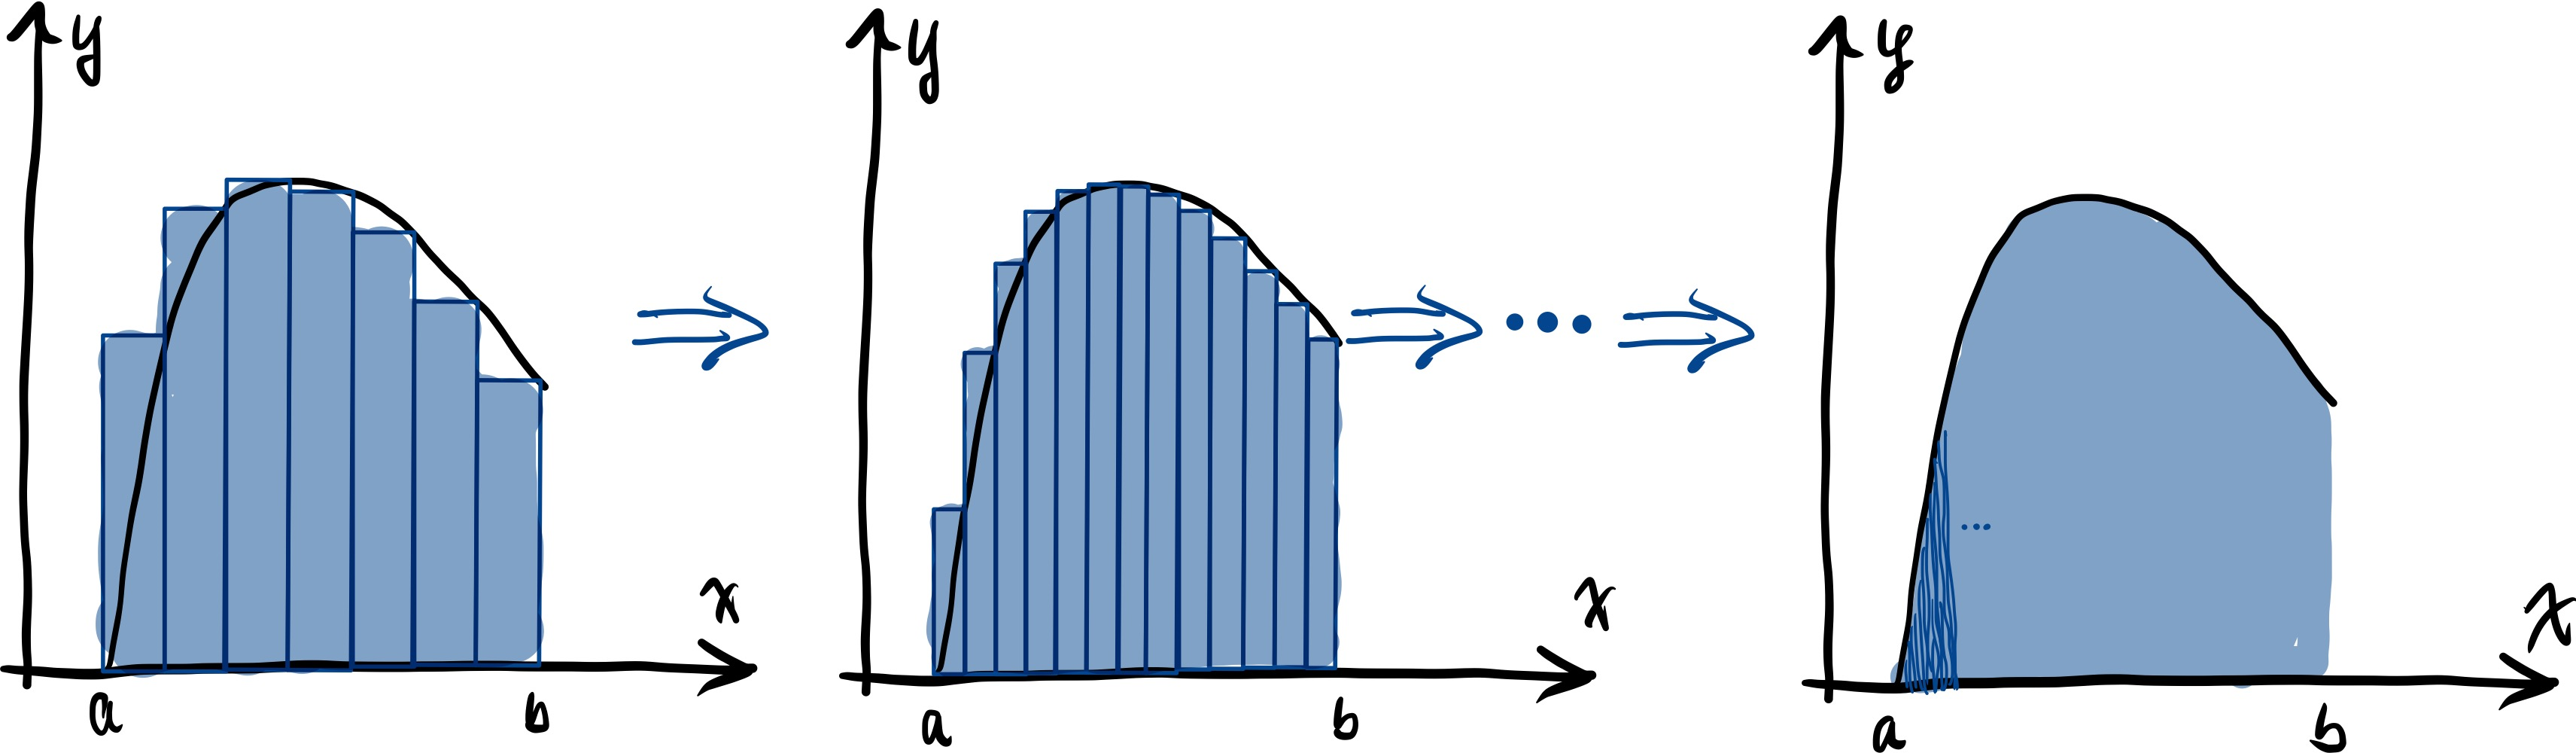
\includegraphics{image-20230906163643414.png}
\caption{image-20230906163643414}
\end{figure}

正式一点的, 我们把这些矩形面积和称作黎曼和 (Riemann sum): \[
\sum_{i=0}^{i=n-1}f(\xi_i)(x_{i-1}-x_i),
\] 其中 \(x_{i-1}\le\xi_i\le x_i\). 当分割不断变得更加精细,
黎曼和最终趋向的值, 我们称其为函数 \(f(x)\) 在区间 \([a,b]\)
的\textbf{定积分} (definite integral), 暂时将这个值记作 \(I\),
对于任意的 \(\epsilon>0\) 都有 \(\delta>0\) 使得: 对于任意的分割,
子区间的数量 \(n<\delta\), 以及任意选择的每一个 \(\xi_i\) , 我们有: \[
\left|\sum_{i=0}^{i=n-1}f(\xi_i)(x_{i-1}-x_i)-I\right|<\epsilon.
\] 我们可以将定积分定义为, \[
\boxed{I=\lim_{n\rightarrow\infty}\sum_{i=0}^nf(\xi_i)(x_{i+1}-x_i).}
\] 令 \(\Delta x:=x_{i+1}-x_i\), 这样一来,
上面取子区间的数量趋向无穷的极限一定程度上等价于每个子区间的''宽度''趋向于无穷小,
于是在这个极限下 \(\Delta x\) 变成了一个无穷小量, 即
\(\Delta x\rightarrow \mathrm{d}x\)\footnote{这个操作在物理中经常出现,
  要很熟悉这种找到有限的变化之间的关系, 然后令它变为无穷小量这样的操作.}.
对此, 莱布尼兹 (Leibniz) 发明了一个定积分的标记,
他将一个''S''拉长表示这种特殊的''求和'', 于是上面的定积分我们便通常写作
\[
\boxed{\int_a^bf(x)\mathrm{d}x.}
\] 有一点要注意的是, 这个积分之和函数本身 \(f\), 积分的区间 \([a,b]\)
相关, 和积分对象 \(x\) 无关, 所以将定积分的积分对象由 \(x\)
换为其他任意字母, 得到的结果是不变的. 于是在这种情况下, 像 \(x\)
这样出现在公式中, 但又不实际太多地参与到运算中的变量,
我们称之为虚拟变量/哑变量 (dummy variable,
个人认为傀儡变量更信雅达一些).

\begin{quote}
很多初学者最早在接触积分的时候, 会忘记最后的 \(\mathrm{d}x\),
本人最初的理解是, 这个 \(\mathrm{d}x\) 是用来表示积分对象是 \(x\);
但从函数图像面积这样的几何角度出发, 这个 \(\mathrm{d}x\)
事实上是每一个子区间面积的''底'', 因此这个 \(\mathrm{d}x\)
是不能被省略的.
\end{quote}

\textbf{更加严格的版本 - 选读}

对于某一个特定的分割, 在子区间 \([x_{i-1},x_i]\) 中, 令 \[
\begin{gather*}
M_i:=\sup \left(f(x)\right),\\
m_i:=\inf \left(f(x)\right).
\end{gather*}
\]

\begin{quote}
这里 \(\sup\) 和 \(\inf\) 全写是 supremum 和 infimum,
中文分别是上确界和下确界, 和最大值 \(\max\) 和最小值 \(\min\) 很像,
区别在于, 例如在某个区间内, 若 \(f(x)\le \eta\), 我们可以说
\(\eta=\max \left(f(x)\right)=\sup \left(f(x)\right)\), 但若
\(f(x)<\eta\), 我们只能说 \(\eta=\sup \left(f(x)\right)\) 因为
\(\max \left(f(x)\right)\) 取不到 \(\eta\).
\end{quote}

再令 \[
\begin{gather*}
U:=\sum M_i\Delta_i,\\
L:=\sum m_i\Delta_i,
\end{gather*}
\] 相当于某一个特定的分割下, 黎曼和的上限和下限, 最后令 \[
\overline{\int_a^b}f(x)\mathrm{d}x:=\inf U,\\
\underline{\int_a^b}f(x)\mathrm{d}x:=\sup L,
\] 即所有分割下, \(U\) 的下限和 \(L\) 的上限 (上限的下限和下限的上限,
lol), 分别称他们为黎曼上积分和黎曼下积分.
若一个函数在一个区间内黎曼上积分和下积分相等,
我们就说这个函数在这个区间内是黎曼可积的 (Riemann integrable),
积分的值记作 \(\int_a^bf(x)\mathrm{d}x\).
